\chapter{HUẤN LUYỆN VÀ TỐI ƯU HÓA MÔ HÌNH (MODEL TRAINING)}
Dựa trên tập đặc trưng đã được tối ưu hóa từ chương trước, nghiên cứu tiến hành huấn luyện các mô hình dự báo nồng độ PM2.5 cho khung thời gian 24 giờ tới ($t+24$). Quy trình được thực hiện qua hai giai đoạn: thiết lập mô hình cơ sở (Baseline) và tối ưu hóa siêu tham số chuyên sâu.
\section{Thiết lập mô hình cơ sở (Baseline Models)}
Giai đoạn đánh giá Baseline nhằm xác định năng lực dự báo tiềm năng của các kiến trúc thuật toán khi sử dụng các thiết lập tham số mặc định hoặc tiêu chuẩn.
\subsection{Nhóm mô hình học máy dạng cây (Tree-based Models)}
Nghiên cứu lựa chọn ba thuật toán Ensemble Learning phổ biến dựa trên cấu trúc cây quyết định để làm mô hình cơ sở. Các mô hình này được huấn luyện trên tập dữ liệu nguyên bản (original scale) do đặc tính không nhạy cảm với thang đo của cấu trúc phân nhánh:
\begin{itemize}
    \item \textbf{Random Forest (RF):} Sử dụng cơ chế \textit{Bagging} với 200 thực thể cây (\texttt{n\_estimators}) và độ sâu tối đa 20 lớp nhằm kiểm soát khả năng học thuộc lòng của mô hình.
    \item \textbf{XGBoost (XGB):} Thuật toán \textit{Gradient Boosting} sử dụng phương pháp biểu đồ (\textit{Histogram method}) để tăng tốc độ huấn luyện và thực hiện lấy mẫu đặc trưng ngẫu nhiên (\texttt{colsample\_bytree}) ở mức 0.9.
    \item \textbf{LightGBM (LGBM):} Một biến thể Boosting tối ưu về hiệu năng tính toán, sử dụng chiến lược phát triển cây theo chiều sâu lá (\textit{Leaf-wise}) với tốc độ học $\eta = 0.05$.
\end{itemize}
Kết quả đánh giá trên tập Kiểm tra (Testing set) được tổng hợp trong Bảng \ref{tab:tree_baseline_metrics} và Hình \ref{fig:tree_models_test_metrics_bar}.
\begin{table}[H]
    \centering
    \caption{Hiệu năng của các mô hình Tree-based Baseline trên tập Kiểm tra}
    \label{tab:tree_baseline_metrics}
    \begin{tabular}{|l|c|c|c|}
    \hline
    \textbf{Mô hình} & \textbf{RMSE ($\mu g/m^3$)} & \textbf{MAE ($\mu g/m^3$)} & \textbf{MAPE (\%)} \\ \hline
    Random Forest    & 21,12 & 15,08 & 44,76 \\ \hline
    XGBoost          & \textbf{19,93} & \textbf{14,67} & \textbf{42,92} \\ \hline
    LightGBM         & 20,38 & 14,89 & 43,46 \\ \hline
    \end{tabular}
\end{table}
\begin{figure}[H]
    \centering
    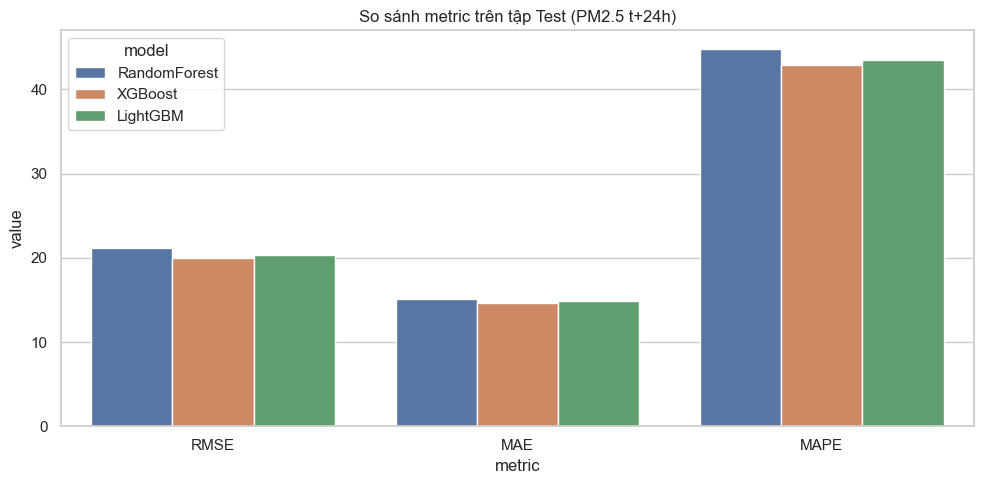
\includegraphics[width=0.85\textwidth]{figure/tree_bar.png}
    \caption{So sánh các chỉ số sai số của nhóm mô hình Tree-based Baseline}
    \label{fig:tree_models_test_metrics_bar}
\end{figure}
Kết quả sơ bộ cho thấy \textbf{XGBoost} thể hiện khả năng dự báo vượt trội nhất ngay cả khi chưa qua tinh chỉnh siêu tham số. Tuy nhiên, sai số MAPE ở mức trên 40\% cho thấy các thiết lập mặc định chưa đủ để mô hình phản ứng linh hoạt với các sự kiện ô nhiễm không khí phức tạp, đặt ra nhu cầu về một quy trình tối ưu hóa chuyên sâu hơn ở giai đoạn sau.

\subsection{Nhóm mô hình thống kê (Statistical Models)}
Khác với nhóm mô hình cây, các mô hình thống kê trong nghiên cứu này tập trung vào việc mô hình hóa cấu trúc tự tương quan (\textit{Auto-correlation}) và các thành phần mùa vụ của chuỗi thời gian. Nghiên cứu thực hiện đánh giá bốn biến thể gồm ARIMA, SARIMA và các phiên bản mở rộng với biến ngoại sinh (ARIMAX, SARIMAX).
\subsubsection{Cấu hình và Tham số cơ sở}
Để thiết lập vạch xuất phát, các mô hình được cấu hình với các tham số bậc tự hồi quy ($p, P$), bậc trung bình trượt ($q, Q$) và tính mùa vụ ($s=24$) nhằm tương ứng với chu kỳ thay đổi theo giờ của PM2.5:
\begin{itemize}
    \item \textbf{ARIMA:} Sử dụng cấu hình cơ bản $(1, 1, 1)$ làm nền tảng, tập trung vào khả năng tự hồi quy và xử lý tính không dừng thông qua lấy sai phân bậc 1.
    \item \textbf{SARIMA:} Mở rộng từ ARIMA với thành phần mùa vụ $(1, 0, 0)_{24}$, giúp mô hình ghi nhớ các quy luật lặp lại hàng ngày (chu kỳ 24 giờ) của PM2.5.
    \item \textbf{ARIMAX/SARIMAX:} Tích hợp thêm các biến ngoại sinh (\textit{Exogenous}) bao gồm top 5 đặc trưng khí tượng (như vận tốc gió, độ ẩm, áp suất) đã qua chọn lọc từ quy trình Feature Selection để cung cấp thêm các tín hiệu vật lý hỗ trợ dự báo.
\end{itemize}
\subsubsection{Chiến lược Ngăn chặn Rò rỉ Dữ liệu (Data Leakage Prevention)}
Trong dự báo chuỗi thời gian, rò rỉ dữ liệu là rủi ro lớn nhất dẫn đến kết quả dự báo "ảo". Nghiên cứu áp dụng quy trình kiểm soát nghiêm ngặt thông qua kỹ thuật \textbf{True 24-Step Walk-Forward Forecast}:
\begin{itemize}
    \item \textbf{Cơ chế Dự báo:} Để dự báo cho thời điểm $t+24$, mô hình chỉ được phép tiếp cận dữ liệu mục tiêu tối đa đến thời điểm $t$. Toàn bộ giá trị từ $t+1$ đến $t+23$ tuyệt đối không xuất hiện trong tập đầu vào (\textit{Endogenous}).
    \item \textbf{Cập nhật Luồng dữ liệu:} Thay vì dự báo tĩnh cho toàn bộ tập Test, nghiên cứu thực hiện vòng lặp rolling. Tại mỗi bước, một quan sát thực tế tại $t$ được \texttt{append} vào lịch sử của mô hình để dự báo cho $t+24$ giờ tiếp sau. Quá trình này không thực hiện huấn luyện lại (\texttt{refit=False}) để đảm bảo tính khách quan của tham số Baseline.
    \item \textbf{Đồng bộ ngoại sinh:} Các biến ngoại sinh tại thời điểm dự báo cũng được đảm bảo là các giá trị khả dụng tại thời điểm thực hiện lệnh dự báo.
\end{itemize}
\subsubsection{Kết quả dự báo Baseline}
Kết quả thu được sau khi hoàn tác biến đổi Logarit (\texttt{expm1}) trên tập Kiểm tra được trình bày trong Bảng \ref{tab:stats_baseline_metrics}.
\begin{table}[H]
    \centering
    \caption{Hiệu năng của các mô hình Thống kê Baseline trên tập Kiểm tra}
    \label{tab:stats_baseline_metrics}
    \begin{tabular}{|l|c|c|c|}
    \hline
    \textbf{Mô hình} & \textbf{RMSE ($\mu g/m^3$)} & \textbf{MAE ($\mu g/m^3$)} & \textbf{MAPE (\%)} \\ \hline
    SARIMA           & 20,38 & 13,75 & \textbf{31,08} \\ \hline
    ARIMAX           & 21,84 & 14,62 & 36,83 \\ \hline
    SARIMAX          & \textbf{18,88} & \textbf{13,49} & 36,70 \\ \hline
    \end{tabular}
\end{table}
Đáng chú ý, mô hình \textbf{SARIMAX} cho kết quả RMSE thấp hơn hẳn so với tất cả các mô hình học máy dạng cây ở giai đoạn Baseline. Điều này khẳng định rằng PM2.5 tại TP.HCM mang tính phụ thuộc thời gian rất mạnh và các biến khí tượng đóng vai trò then chốt trong việc hiệu chỉnh các sai số của dự báo thống kê thuần túy.

\subsection{Nhóm mô hình học sâu (Deep Learning Models)}
Để đối chiếu với các phương pháp học máy truyền thống và thống kê, nghiên cứu triển khai hai kiến trúc mạng nơ-ron hồi tiếp (Recurrent Neural Networks - RNN) phổ biến là \textbf{LSTM} (Long Short-Term Memory) và \textbf{GRU} (Gated Recurrent Unit). Đây là các kiến trúc được thiết kế chuyên biệt để xử lý dữ liệu chuỗi có tính phụ thuộc thời gian phức tạp.
\subsubsection{Cấu trúc mạng và Quy trình huấn luyện}
Các mô hình được xây dựng trên nền tảng thư viện PyTorch với cấu trúc tinh gọn nhằm thiết lập hiệu năng cơ sở:
\begin{itemize}
    \item \textbf{Cấu trúc lớp:} Mỗi mô hình bao gồm 01 lớp RNN (LSTM hoặc GRU) với 64 đơn vị ẩn (\textit{hidden units}), theo sau là một lớp tuyến tính (\textit{Linear layer}) để chuyển đổi không gian đặc trưng về giá trị dự báo nồng độ bụi đơn nhất.
    \item \textbf{Hình dạng dữ liệu (Input Reshaping):} Ma trận đặc trưng phẳng (đã qua chuẩn hóa Z-score ở Chương 3) được biến đổi thành dạng Tensor 3 chiều với kích thước $(\text{Batch}, 1, \text{Features})$. Cách tiếp cận này cho phép mạng RNN trích xuất thông tin từ tập biến trễ đã được làm phẳng trong quy trình Feature Engineering.
    \item \textbf{Cấu hình huấn luyện:} Sử dụng hàm mất mát MSE (\textit{Mean Squared Error}) và thuật toán tối ưu hóa Adam với tốc độ học truyền thống 0,001. Mô hình thực hiện huấn luyện qua 50 chu kỳ (\textit{epochs}) với kích thước lô 64 để đảm bảo sự hội tụ ổn định của gradient.
\end{itemize}
\subsubsection{Kết quả dự báo Baseline}
Hiệu năng của các mô hình học sâu trên tập Kiểm tra (sau khi hoàn tác log) được trình bày trong Bảng \ref{tab:dl_baseline_metrics}.
\begin{table}[H]
    \centering
    \caption{Hiệu năng của các mô hình Deep Learning Baseline trên tập Kiểm tra}
    \label{tab:dl_baseline_metrics}
    \begin{tabular}{|l|c|c|c|}
    \hline
    \textbf{Mô hình} & \textbf{RMSE ($\mu g/m^3$)} & \textbf{MAE ($\mu g/m^3$)} & \textbf{MAPE (\%)} \\ \hline
    LSTM             & \textbf{18,64} & \textbf{13,10} & \textbf{33,70} \\ \hline
    GRU              & 19,24 & 13,45 & 34,55 \\ \hline
    \end{tabular}
\end{table}

\begin{figure}[H]
    \centering
    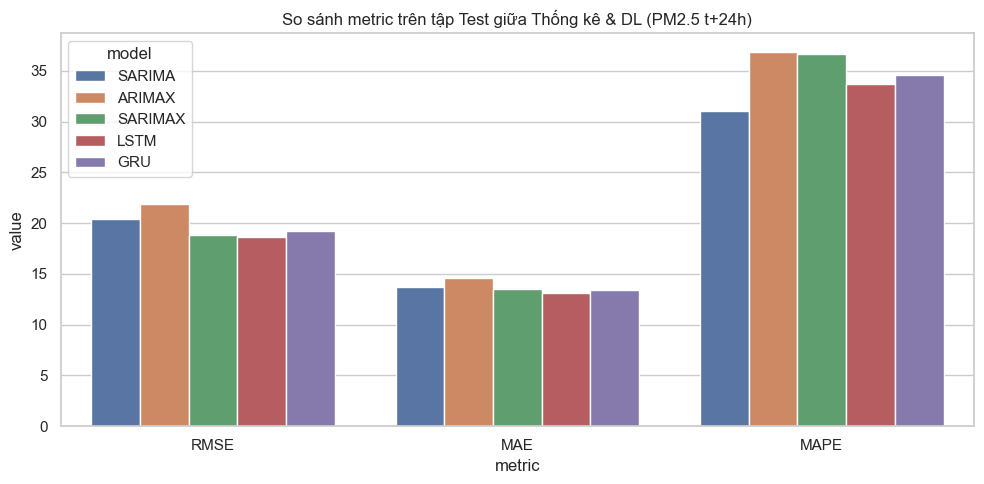
\includegraphics[width=0.85\textwidth]{figure/output.png}
    \caption{So sánh sai số giữa các mô hình Thống kê và Deep Learning cơ sở}
    \label{fig:stats_baseline_bar}
\end{figure}

\textbf{LSTM} ghi nhận kết quả tốt nhất trong toàn bộ nhóm Baseline (Tree, Stats và DL) với mức RMSE thấp nhất (18,64). Điều này minh chứng cho khả năng vượt trội của kiến trúc Long Short-Term Memory trong việc nắm bắt các phụ thuộc phi tuyến trong chuỗi thời gian PM2.5. GRU cho kết quả bám đuổi sát sao nhưng chưa tối ưu bằng, có thể do khả năng kiểm soát luồng thông tin qua các cổng (\textit{gates}) của LSTM phù hợp hơn với đặc tính dữ liệu khí tượng đa biến hiện có.


% Trình bày việc khởi tạo SARIMA, XGBoost, LightGBM, LSTM, GRU với các tham số mặc định.
\section{Chiến lược Tối ưu hóa Siêu tham số (Tuning Strategy)}
Sau giai đoạn Baseline, nghiên cứu nhận thấy hiện tượng quá khớp (\textit{Overfitting}) xảy ra nghiêm trọng ở nhóm mô hình cây (sai số tập Huấn luyện thấp hơn gấp nhiều lần các tập còn lại). Do đó, giai đoạn tối ưu hóa tập trung vào việc cân bằng giữa năng lực học và khả năng tổng quát hóa của mô hình thông qua việc rà soát không gian tham số có hệ thống.
\subsection{Tối ưu hóa nhóm mô hình cây (Tree-based Models)}
Quy trình tối ưu hóa được thực hiện thông qua thuật toán tìm kiếm ngẫu nhiên (\texttt{RandomizedSearchCV}) kết hợp với cơ chế kiểm định chéo chuỗi thời gian (\texttt{TimeSeriesSplit}) với 5 lần lặp (\textit{folds}). Phương pháp này đảm bảo tính nhân quả, tránh việc sử dụng thông tin từ "tương lai" để rà soát tham số.
Chiến lược tinh chỉnh tập trung vào cơ chế điều tiết (\textit{Regularization-First}):
\begin{itemize}
    \item \textbf{Kiểm soát độ sâu:} Giới hạn chặt chẽ tham số \texttt{max\_depth} để tránh việc các cây quyết định chia nhánh quá chi tiết vào các điểm nhiễu.
    \item \textbf{Tăng ngưỡng điều kiện:} Nâng cao các thông số \texttt{min\_samples\_leaf} (cho RF/LGBM) và \texttt{min\_child\_weight} (cho XGB) nhằm yêu cầu mỗi lá cây phải chứa đủ lượng mẫu đại diện nhất định mới được phép phân nhánh.
    \item \textbf{Áp dụng hình phạt trọng số:} Sử dụng các hệ số \texttt{reg\_alpha} ($L_1$) và \texttt{reg\_lambda} ($L_2$) để trực tiếp triệt tiêu hoặc giảm thiểu trọng số của các đặc trưng ít đóng góp vào phương sai chung.
\end{itemize}
Không gian rà soát siêu tham số được đề xuất chi tiết trong Bảng \ref{tab:tree_search_space}.
\begin{table}[H]
    \centering
    \caption{Không gian tìm kiếm siêu tham số cho nhóm mô hình cây}
    \label{tab:tree_search_space}
    \begin{tabular}{|l|l|l|}
    \hline
    \textbf{Mô hình} & \textbf{Tham số tinh chỉnh} & \textbf{Miền giá trị tìm kiếm} \\ \hline
    \multirow{3}{*}{\shortstack{Random \\ Forest}} & \texttt{max\_depth} & [5, 7, 10, 12, None] \\
                                   & \texttt{min\_samples\_leaf} & [4, 8, 16, 32] \\
                                   & \texttt{max\_features} & [sqrt, log2, 0,5, 0,7] \\ \hline
    \multirow{4}{*}{XGBoost}       & \texttt{learning\_rate} & [0,01, 0,03, 0,05, 0,08] \\
                                   & \texttt{max\_depth} & [3, 4, 5, 6] \\
                                   & \texttt{reg\_alpha / reg\_lambda} & [0, 0,1, 1,0, 5,0, 10,0] \\
                                   & \texttt{min\_child\_weight} & [3, 5, 10, 20] \\ \hline
    \multirow{4}{*}{LightGBM}      & \texttt{num\_leaves} & [15, 31, 47, 63] \\
                                   & \texttt{min\_child\_samples} & [10, 20, 50, 100] \\
                                   & \texttt{colsample\_bytree} & [0,6, 0,7, 0,8, 0,9] \\
                                   & \texttt{n\_estimators} & [300, 500, 800] \\ \hline
    \end{tabular}
\end{table}
Sau khi tìm được bộ tham số tối ưu thông qua CV trên tập Huấn luyện, mô hình sẽ được huấn luyện lại (\textit{Refit}) trên tập dữ liệu gộp (Huấn luyện + Kiểm thử phát triển) để tận dụng tối đa lượng thông tin trước khi chuyển sang giai đoạn đánh giá cuối cùng.

\subsection{Tối ưu hóa mô hình thống kê (Statistical Models Tuning)}
Việc tối ưu hóa các mô hình họ ARIMA đòi hỏi quy trình tuyển chọn biến dữ liệu và tham số bậc tự hồi quy khắt khe hơn nhằm đảm bảo tính ổn định và ý nghĩa thống kê của các hệ số hồi quy.
\subsubsection{Sàng lọc biến ngoại sinh và Kiểm định tính dừng}
Đối với các biến thể ARIMAX và SARIMAX, nghiên cứu thực hiện quy trình chọn lọc đặc trưng ngoại sinh (\textit{Exogenous Selection}) qua hai giai đoạn:
\begin{itemize}
    \item \textbf{Tương quan Spearman:} Xác định các biến khí tượng có mối quan hệ đơn điệu mạnh với nồng độ PM2.5 định hướng tương lai.
    \item \textbf{Kiểm định nhân quả Granger (Granger Causality):} Đây là bước then chốt để xác nhận xem các biến khí tượng tại thời điểm $t$ có thực sự mang thông tin tiên lượng cho PM2.5 tại $t+24$ hay không. Chỉ các biến vượt qua ngưỡng $p < 0,05$ mới được đưa vào ma trận ngoại sinh.
    \item \textbf{Kiểm định ADF:} Áp dụng kiểm định Augmented Dickey-Fuller để xác định bậc sai phân ($d$), đảm bảo chuỗi trung bình trượt là dừng (\textit{Stationary}) trước khi rà soát các tham số khác.
\end{itemize}
\subsubsection{Thuật toán rà soát Stepwise và Tiêu chuẩn AIC}
Do tính chất phức tạp của chu kỳ mùa vụ ($m=24$), nghiên cứu sử dụng thuật toán tìm kiếm từng bước (\textit{Stepwise Search}) thay vì Grid Search toàn phần để tối ưu hóa thời gian tính toán. Tiêu chuẩn thông tin Akaike (AIC) được chọn làm hàm mục tiêu chính nhằm tìm ra "điểm ngọt" giữa độ chính xác và độ phức tạp của mô hình (Bảng \ref{tab:stats_search_space}).
\begin{table}[H]
    \centering
    \caption{Không gian rà soát thông số cấu hình dòng ARIMA}
    \label{tab:stats_search_space}
    \begin{tabular}{|l|l|l|}
    \hline
    \textbf{Thành phần} & \textbf{Tham số} & \textbf{Miền giá trị rà soát} \\ \hline
    Tự hồi quy (Non-seasonal) & $p, q$ & [0, 1, 2, 3] \\
    Sai phân (Differencing)   & $d$    & [0, 1] (Dựa trên ADF) \\
    Tự hồi quy (Seasonal)     & $P, Q$ & [0, 1, 2] \\
    Chu kỳ mùa vụ             & $m$    & 24 (Chu kỳ ngày) \\
    Tiêu chuẩn tối ưu         & Hàm mục tiêu & Minimize AIC \\ \hline
    \end{tabular}
\end{table}
Sau khi tìm được bộ tham số tối ưu, mô hình được kiểm định phần dư bằng kiểm định \textbf{Ljung-Box} để đảm bảo không còn tính tự tương quan thừa, xác nhận mô hình đã khai thác tối đa tín hiệu từ dữ liệu lịch sử.

\subsection{Tối ưu hóa nhóm mô hình học sâu (Deep Learning Models Tuning)}
Khác với các mô hình cây hay thống kê, việc tối ưu hóa nhóm học sâu không chỉ dừng lại ở các tham số số học mà còn mở rộng ra việc tinh chỉnh toàn bộ cấu trúc (\textit{Architecture Search}) của mạng nơ-ron hồi quy.
\subsubsection{Kiến trúc Dynamic RNN và Cơ chế học hai chiều}
Nghiên cứu thiết lập một cấu trúc mạng linh hoạt (\textit{DynamicRNN}) được xây dựng trên nền tảng PyTorch, cho phép rà soát đồng thời các biến thể kiến trúc khác nhau:
\begin{itemize}
    \item \textbf{Cấu trúc chồng phối (Stacked Layers):} Thử nghiệm việc xếp chồng các lớp RNN để tăng khả năng trích xuất đặc trưng bậc cao.
    \item \textbf{Học hai chiều (Bidirectional RNN):} Cho phép mô hình học các mẫu dữ liệu theo cả chiều thuận và chiều nghịch của chuỗi thời gian, giúp tăng cường khả năng nắm bắt ngữ cảnh cho dữ liệu PM2.5.
    \item \textbf{Lớp giải mã (MLP Decoder):} Phần đầu ra được thiết kế gồm các lớp Tuyến tính (\textit{Linear Layers}) kết hợp với hàm kích hoạt ReLU và Dropout để thực hiện suy luận cuối cùng.
\end{itemize}
\subsubsection{Cơ chế ổn định huấn luyện và Không gian rà soát}
Để đảm bảo quá trình hội tụ tối ưu và tránh hiện tượng quá khớp, các "Plugins" trợ giúp huấn luyện được tích hợp (Bảng \ref{tab:dl_search_space}):
\begin{itemize}
    \item \textbf{Early Stopping:} Tự động dừng huấn luyện sau 10 Epoch nếu sai số trên tập kiểm thử phát triển không giảm, giúp bảo toàn trạng thái tốt nhất của mô hình.
    \item \textbf{ReduceLROnPlateau:} Cơ chế giảm tốc độ học (\textit{Learning rate}) một cách chủ động khi mô hình rơi vào vùng bão hòa, hỗ trợ việc tìm kiếm cực tiểu toàn cục chính xác hơn.
\end{itemize}
\begin{table}[H]
    \centering
    \caption{Không gian rà soát thông số cấu hình mạng Deep Learning}
    \label{tab:dl_search_space}
    \begin{tabular}{|l|l|}
    \hline
    \textbf{Thành phần cấu trúc} & \textbf{Miền giá trị rà soát} \\ \hline
    Loại mạng RNN                & [LSTM, GRU] \\
    Số lượng nút ẩn (Hidden Size) & [64, 128] \\
    Số lớp chồng phối (Layers)   & [1, 2] \\
    Cơ chế học                   & [Unidirectional, Bidirectional] \\
    Tỉ lệ Dropout                & [0,1, 0,3] \\ \hline
    Tốc độ học (Learning Rate)   & Khởi đầu $1 \times 10^{-3}$ (Kết hợp Scheduler) \\
    Chống quá khớp (Weight Decay)& $1 \times 10^{-5}$ ($L_2$ Regularization) \\ \hline
    \end{tabular}
\end{table}